%==============================================================================
% tento soubor pouzijte jako zaklad
% this file should be used as a base for the thesis
% Autoři / Authors: 2008 Michal Bidlo, 2016 Jaroslav Dytrych
% Kontakt pro dotazy a připomínky: dytrych@fit.vutbr.cz
% Contact for questions and comments: dytrych@fit.vutbr.cz
%==============================================================================
% kodovani: UTF-8 (zmena prikazem iconv, recode nebo cstocs)
% encoding: UTF-8 (you can change it by command iconv, recode or cstocs)
%------------------------------------------------------------------------------
% zpracování / processing: make, make pdf, make clean
%==============================================================================
% Soubory, které je nutné upravit: / Files which have to be edited:
%   projekt-20-literatura-bibliography.bib - literatura / bibliography
%   projekt-01-kapitoly-chapters.tex - obsah práce / the thesis content
%   projekt-30-prilohy-appendices.tex - přílohy / appendices
%==============================================================================
\documentclass[slovak]{fitthesis}
%\documentclass[slovak, cprint]{fitthesis}

% bez zadání - pro začátek práce, aby nebyl problém s překladem
%\documentclass[english]{fitthesis} % without assignment - for the work start to avoid compilation problem
%\documentclass[zadani]{fitthesis} % odevzdani do wisu - odkazy jsou barevné
%\documentclass[english,zadani]{fitthesis} % for submission to the IS FIT - links are color
%\documentclass[zadani,print]{fitthesis} % pro tisk - odkazy jsou černé
%\documentclass[zadani,cprint]{fitthesis} % pro barevný tisk - odkazy jsou černé, znak VUT barevný
%\documentclass[english,zadani,print]{fitthesis} % for the color print - links are black
%\documentclass[english,zadani,cprint]{fitthesis} % for the print - links are black, logo is color
% * Je-li práce psaná v anglickém jazyce, je zapotřebí u třídy použít 
%   parametr english následovně:
%   If thesis is written in english, it is necessary to use 
%   parameter english as follows:
%      \documentclass[english]{fitthesis}
% * Je-li práce psaná ve slovenském jazyce, je zapotřebí u třídy použít 
%   parametr slovak následovně:
%   If the work is written in the Slovak language, it is necessary 
%   to use parameter slovak as follows:
%      \documentclass[slovak]{fitthesis}
% * Je-li práce psaná v anglickém jazyce se slovenským abstraktem apod., 
%   je zapotřebí u třídy použít parametry english a enslovak následovně:
%   If the work is written in English with the Slovak abstract, etc., 
%   it is necessary to use parameters english and enslovak as follows:
%      \documentclass[english,enslovak]{fitthesis}

% Základní balíčky jsou dole v souboru šablony fitthesis.cls
% Basic packages are at the bottom of template file fitthesis.cls
% zde můžeme vložit vlastní balíčky / you can place own packages here

% Kompilace po částech (rychlejší, ale v náhledu nemusí být vše aktuální)
% Compilation piecewise (faster, but not all parts in preview will be up-to-date)
\usepackage{subfiles}

% Nastavení cesty k obrázkům
% Setting of a path to the pictures
%\graphicspath{{obrazky-figures/}{./obrazky-figures/}}
%\graphicspath{{obrazky-figures/}{../obrazky-figures/}}

%---rm---------------
\renewcommand{\rmdefault}{lmr}%zavede Latin Modern Roman jako rm / set Latin Modern Roman as rm
%---sf---------------
\renewcommand{\sfdefault}{qhv}%zavede TeX Gyre Heros jako sf
%---tt------------
\renewcommand{\ttdefault}{lmtt}% zavede Latin Modern tt jako tt

% vypne funkci šablony, která automaticky nahrazuje uvozovky,
% aby nebyly prováděny nevhodné náhrady v popisech API apod.
% disables function of the template which replaces quotation marks
% to avoid unnecessary replacements in the API descriptions etc.
\csdoublequotesoff

% =======================================================================
% balíček "hyperref" vytváří klikací odkazy v pdf, pokud tedy použijeme pdflatex
% problém je, že balíček hyperref musí být uveden jako poslední, takže nemůže
% být v šabloně
% "hyperref" package create clickable links in pdf if you are using pdflatex.
% Problem is that this package have to be introduced as the last one so it 
% can not be placed in the template file.
\ifWis
\ifx\pdfoutput\undefined % nejedeme pod pdflatexem / we are not using pdflatex
\else
  \usepackage{color}
  \usepackage[unicode,colorlinks,hyperindex,plainpages=false,pdftex]{hyperref}
  \definecolor{links}{rgb}{0.4,0.5,0}
  \definecolor{anchors}{rgb}{1,0,0}
  \def\AnchorColor{anchors}
  \def\LinkColor{links}
  \def\pdfBorderAttrs{/Border [0 0 0] }  % bez okrajů kolem odkazů / without margins around links
  \pdfcompresslevel=9
\fi
\else % pro tisk budou odkazy, na které se dá klikat, černé / for the print clickable links will be black
\ifx\pdfoutput\undefined % nejedeme pod pdflatexem / we are not using pdflatex
\else
  \usepackage{color}
  \usepackage[unicode,colorlinks,hyperindex,plainpages=false,pdftex,urlcolor=black,linkcolor=black,citecolor=black]{hyperref}
  \definecolor{links}{rgb}{0,0,0}
  \definecolor{anchors}{rgb}{0,0,0}
  \def\AnchorColor{anchors}
  \def\LinkColor{links}
  \def\pdfBorderAttrs{/Border [0 0 0] } % bez okrajů kolem odkazů / without margins around links
  \pdfcompresslevel=9
\fi
\fi
% Řešení problému, kdy klikací odkazy na obrázky vedou za obrázek
% This solves the problems with links which leads after the picture
\usepackage[all]{hypcap}
\usepackage{subcaption}
\usepackage{varwidth}
\usepackage{amsmath}
\usepackage{kbordermatrix,blkarray}

\usepackage[Algoritmus]{algorithm}
\usepackage[noend]{algpseudocode}


\captionsetup{compatibility=false}

% Informace o práci/projektu / Information about the thesis
%---------------------------------------------------------------------------
\projectinfo{
  %Prace / Thesis
  project={BP},            %typ práce BP/SP/DP/DR  / thesis type (SP = term project)
  year={2018},             % rok odevzdání / year of submission
  date=\today,             % datum odevzdání / submission date
  %Nazev prace / thesis title
  title.cs={Webová aplikácia na vzdialenú správu systému Fitcrack},  % název práce v češtině či slovenštině (dle zadání) / thesis title in czech language (according to assignment)
  title.en={Web Application for Remote Administration of Fitcrack System}, % název práce v angličtině / thesis title in english
  %title.length={14.5cm}, % nastavení délky bloku s titulkem pro úpravu zalomení řádku (lze definovat zde nebo níže) / setting the length of a block with a thesis title for adjusting a line break (can be defined here or below)
  %Autor / Author
  author.name={Matúš},   % jméno autora / author name
  author.surname={Múčka},   % příjmení autora / author surname 
  %author.title.p={Bc.}, % titul před jménem (nepovinné) / title before the name (optional)
  %author.title.a={Ph.D.}, % titul za jménem (nepovinné) / title after the name (optional)
  %Ustav / Department
  department={UIFS}, % doplňte příslušnou zkratku dle ústavu na zadání: UPSY/UIFS/UITS/UPGM / fill in appropriate abbreviation of the department according to assignment: UPSY/UIFS/UITS/UPGM
  % Školitel / supervisor
  supervisor.name={Radek},   % jméno školitele / supervisor name 
  supervisor.surname={Hranický},   % příjmení školitele / supervisor surname
  supervisor.title.p={Ing.},   %titul před jménem (nepovinné) / title before the name (optional)
  %supervisor.title.a={Ph.D.},    %titul za jménem (nepovinné) / title after the name (optional)
  % Klíčová slova / keywords
  keywords.cs={REST, Fitcrack, API, backend}, % klíčová slova v českém či slovenském jazyce / keywords in czech or slovak language
  keywords.en={REST, Fitcrack, API, backend}, % klíčová slova v anglickém jazyce / keywords in english
  % Abstrakt / Abstract
  abstract.cs={Táto práca rieši vzdialenú komunikáciu so systémom na distribuovanú obnovu hesiel - Fitcrack. Zameral som sa na vylepšenie súčasného riešenia. Okrem zvýšenia bezpečnosti a rýchlejšej odozvy, návrh riešenia uvedený v~tejto práci ponúka aj podporu autentifikácie užívateľov a ich oprávnení. Systém bude automaticky generovať dokumentáciu pri zmene zdrojových kódov. V~riešení bola použitá architektúra REST (viď \ref{rest}). Táto architektúra umožňuje oddeliť aplikačnú logiku od databázového systému, a tým pádom umožniť komunikáciu s~aplikáciami pomocou zasielanie správ. Vďaka tomu je možné systém Fitcrack ovládať z~rôznych prostredí pomocou jednoduchých dotazov protokolu HTTP. V~mojej práci som navrhol systém, ktorý zrýchli komunikáciu so systémom Fitcrack, zlepší zabezpečenie a pridá do systému vylepšenia ako podpora viacerých užívateľov a ich oprávnení.

  
  }, % abstrakt v českém či slovenském jazyce / abstract in czech or slovak language
  abstract.en={This bachelor’s thesis resolves remote communication with distributed password recovery system - Fitcrack. I~aimed to improve a current implemented solution. In addition to security improvement and faster responses, the design of solution presented in this work offers support for user authentication and authorization. The system automatically generate documentation when source code changes. REST (see \ref{rest}) architecture was used in this solution. This architecture allows to separate the application logic and the database system which consequently allows application communication by sending messages. Because of that, it is possible to control Fitcrack from different environments using simple HTTP queries. I~designed the system that accelerates communication with Fitcrack, refines security and adds improvements such as support for multiple user privileges.}, % abstrakt v anglickém jazyce / abstract in english
  % Prohlášení (u anglicky psané práce anglicky, u slovensky psané práce slovensky) / Declaration (for thesis in english should be in english)
  declaration={Prehlasujem, že tento semestrálny projekt som vypracoval samostatne pod vedením pána inžiniera Radka Hranického.
  Uviedol som všetky literárne zdroje a publikácie, z~ktorých som čerpal.
  },
  %declaration={Hereby I declare that this bachelor's thesis was prepared as an original author’s work under the supervision of Mr. X
% The supplementary information was provided by Mr. Y
% All the relevant information sources, which were used during preparation of this thesis, are properly cited and included in the list of references.},
  % Poděkování (nepovinné, nejlépe v jazyce práce) / Acknowledgement (optional, ideally in the language of the thesis)
  acknowledgment={Ďakujem Ing. Radkovi Hranickému za odbornú pomoc a vedenie pri vypracovávaní tejto práce.},
  %acknowledgment={Here it is possible to express thanks to the supervisor and to the people which provided professional help
%(external submitter, consultant, etc.).},
  % Rozšířený abstrakt (cca 3 normostrany) - lze definovat zde nebo níže / Extended abstract (approximately 3 standard pages) - can be defined here or below
  %extendedabstract={Do tohoto odstavce bude zapsán rozšířený výtah (abstrakt) práce v českém (slovenském) jazyce.},
  %faculty={FIT}, % FIT/FEKT/FSI/FA/FCH/FP/FAST/FAVU/USI/DEF
  faculty.cs={Fakulta informačních technologií}, % Fakulta v češtině - pro využití této položky výše zvolte fakultu DEF / Faculty in Czech - for use of this entry select DEF above
  faculty.en={Faculty of Information Technology}, % Fakulta v angličtině - pro využití této položky výše zvolte fakultu DEF / Faculty in English - for use of this entry select DEF above
  department.cs={Ústav informačních systémů}, % Ústav v češtině - pro využití této položky výše zvolte ústav DEF nebo jej zakomentujte / Department in Czech - for use of this entry select DEF above or comment it out
  department.en={
Department of Information Systems} % Ústav v angličtině - pro využití této položky výše zvolte ústav DEF nebo jej zakomentujte / Department in English - for use of this entry select DEF above or comment it out
}

% Rozšířený abstrakt (cca 3 normostrany) - lze definovat zde nebo výše / Extended abstract (approximately 3 standard pages) - can be defined here or above
%\extendedabstract{Do tohoto odstavce bude zapsán výtah (abstrakt) práce v českém (slovenském) jazyce.}

% nastavení délky bloku s titulkem pro úpravu zalomení řádku - lze definovat zde nebo výše / setting the length of a block with a thesis title for adjusting a line break - can be defined here or above
%\titlelength{14.5cm}


% řeší první/poslední řádek odstavce na předchozí/následující stránce
% solves first/last row of the paragraph on the previous/next page
\clubpenalty=10000
\widowpenalty=10000

\begin{document}
  % Vysazeni titulnich stran / Typesetting of the title pages
  % ----------------------------------------------
  \maketitle
  % Obsah
  % ----------------------------------------------
  \setlength{\parskip}{0pt}

  {\hypersetup{hidelinks}\tableofcontents}
  
  % Seznam obrazku a tabulek (pokud prace obsahuje velke mnozstvi obrazku, tak se to hodi)
  % List of figures and list of tables (if the thesis contains a lot of pictures, it is good)
  \ifczech
    \renewcommand\listfigurename{Seznam obrázků}
  \fi
  \ifslovak
    \renewcommand\listfigurename{Zoznam obrázkov}
  \fi
  % \listoffigures
  
  \ifczech
    \renewcommand\listtablename{Seznam tabulek}
  \fi
  \ifslovak
    \renewcommand\listtablename{Zoznam tabuliek}
  \fi
  % \listoftables 

  \ifODSAZ
    \setlength{\parskip}{0.5\bigskipamount}
  \else
    \setlength{\parskip}{0pt}
  \fi

  % vynechani stranky v oboustrannem rezimu
  % Skip the page in the two-sided mode
  \iftwoside
    \cleardoublepage
  \fi

  % Text prace / Thesis text
  % ----------------------------------------------
  %\input{chapters/projekt-01-uvod}

\chapter{Úvod}\label{uvod}
V~súčasnosti je používanie aplikačného protokolu HTTP pre sieťový prenos textových dát v~rámci služby World Wide Web (WWW) veľmi rozšírené. Spoločne s~elektronickou poštou je HTTP najviac používaným protokolom, ktorý sa zaslúžil o~obrovský rozmach internetu v~posledných rokoch. Jedným z~autorov protokolu HTTP je Roy Fielding, ktorý vo svojej dizertačnej práci opisuje Representation State Transfer (REST). REST je architektúra, ktorá poskytuje obecné rozhranie pre vzdialené aplikácie, ktoré komunikujú cez sieť. Napriek tomu, že REST nie je určený priamo pre HTTP, je takmer vždy spojovaný s~týmto protokolom.

V~tejto práci popisujem všeobecný opis a implementáciu aplikačné rozhranie spĺňajúce zásady architektúry REST (viď \ref{zasadyREST}) pre systém Fitcrack. Jedná sa o~výkonný systém na obnovu hesiel, ktorý prerozdeľuje prácu medzi viacero pripojených klientov, a tým pádom zvyšuje výpočetnú silu celého systému (detailnejšie je Fitcrack popísaný v~kapitole \ref{Fitcrack}). Konkrétne sa v~mojej práci zaoberám jeho serverovou časťou, ktorá slúži na správu celého systému. Mojim cieľom je nahradiť súčasné nevyhovujúce riešenie administrácie systému, ktoré bolo navrhnuté len ako prototyp, novým riešením.

Súčasná implementácia je veľmi ťažko rozšíriteľná. Taktiež obsahuje niekoľko bezpečnostných dier. Nové riešenie prináša do systému Fitcrack väčšiu bezpečnosť a rozšíriteľnosť, umožňuje testovanie systému, a vďaka architektúre klient-server znižuje záťaž na serverovú časť systému.

Táto práca pozostáva z~piatich kapitol. Popis systému Fitcrack spolu s~nástrojmi, ktoré využíva sa nachádza v~kapitole \ref{Fitcrack}. Opis využitých technológií, ktoré som pri návrhu nového systému na vzdialenú správu Fitcracku použil, sa nachádza v~kapitole \ref{technologie}. Samotným návrhom riešenia, ktorý je rozdelený do modulov, sa zaoberám v~kapitole \ref{navrh}. V~jednotlivých podkapitolách popisujem každý modul. Nakoniec v~závere hodnotím výsledky mojej práce. 



\chapter{Systém Fitcrack}\label{Fitcrack}
Fitcrack je systém, ktorý slúži na obnovu hesiel. Vďaka tomu že ide o~distribuovaný systém, je možné rozdelovať prácu na predom neobmedzený počet staníc, ktoré môžu byť rozmiestnené po celom svete. Je tvorený  architektúrou klient-server. Serverová časť sa stará o~prerozdeľovanie úloh medzi klientov. Klienti pracujú na výpočte kryptografických hešov a svoje výsledky posielajú na server, kde sa spracujú a vyhodnotia.
\cite{fitcrackSprava}


\section{Hashcat}\label{hashcat}
Hashcat\footnote{\url{https://hashcat.net}} je výkonný nástroj na obnovu hesiel, ktorý využíva technológiu OpenCL. Podporuje viac ako 200 typov kryptografických hešov. O~jeho rýchlostí svedčí aj to, že v~rokoch 2010, 2012, 2014 a 2015, tím, pozostávajúci z~členov vývojárov Hashcatu, získal prvé miesto v~súťaži \textit{Crack Me If you Can}\footnote{\url{http://contest-2010.korelogic.com/team_hashcat.html}}. Žiaľ, tento nástroj sám o~sebe nepodporuje výpočet na viacerých staniciach súčasne.


\section{BOINC} \label{BOINC}
Systém Fitcrack je postavený na voľne šíriteľnom frameworku \textit{Berkeley Open Infrastructure for Network Computing} (BOINC)\footnote{\url{https://boinc.berkeley.edu/}}. Vďaka frameworku BOINC systém Fitcrack distribuuje dielčie úlohy medzi pripojených klientov, na ktorých prebieha pokus o~nájdenia hesla pomocou nástroja Hashcat.

Systém BOINC tvorí server a klienti. Pri distribuovaní výpočetných úloh prebieha komunikácia medzi klientom a serverom prostredníctvom XML správ, ktoré sa prenášajú pomocou protokolu HTTP alebo HTTPS.
Server je hlavnou súčasťou infraštruktúry BOINC. Stará sa o~distribuovanie úloh medzi klientov a spracováva výsledky od užívateľov.
Každý klient sa periodicky dotazuje na server a žiada si novú úlohu. Po prijatí výpočetnej úlohy ju spracuje a výsledok odošle na serverom. Následne žiada o~pridelenie novej úlohy.\cite{boinccitace}


\section{Architektúra systému Fitcrack}
Ako je možné vidieť na obrázku \ref{fig:archFitcrack}, architektúra systému Fitcrack je rozdelená na niekoľko častí. Na obrázku je uvedená zjednodušená architektúra bez niektorých systémov BOINC.

\begin{figure}[h]
    \centering
    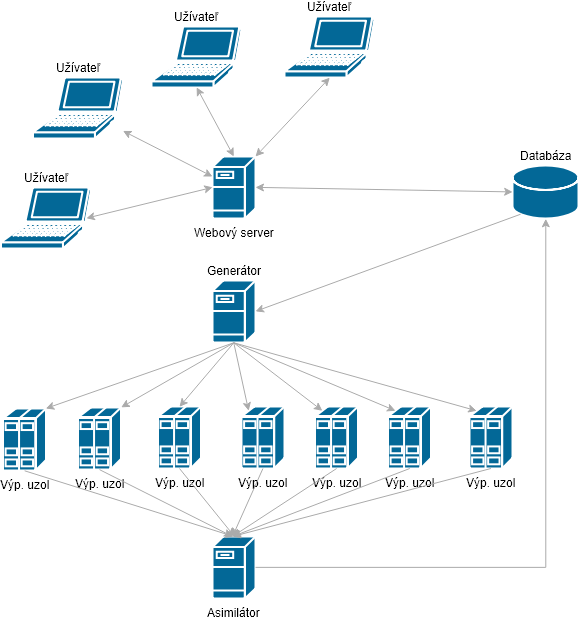
\includegraphics[scale=0.65]{obrazky/FitcrackSystem.png}
    \caption{Architektúra systému Fitcrack}
    \label{fig:archFitcrack}
\end{figure}


\subsection{Webový server}
Cieľom mojej bakalárskej práce je navrhnúť a implementovať webový server, cez ktorý budú môcť užívatelia spravovať celý systém Fitcrack. K webovému serveru môže byť naraz pripojených viacero užívateľov, ktorí vykonávajú rôzne činnosti (analyzovanie výsledkov dokončených úloh, sledovanie aktivity jednotlivých hosťov, pridávanie nových úloh, sledovanie progresu práve prebiehajúcich úloh atď.). Po pripojení užívateľa na webový server cez internetový prehliadač, sa užívateľovi odošle webová aplikácia, ktorá komunikuje so serverom prostredníctvom REST API (viď \ref{rest}). Prostredníctvom webovej aplikácie je možné do systému pridávať nové úlohy, monitorovať prebiehajúce, analyzovať dokončené úlohy, monitorovať správanie hosťov a podobne. Viac o návrhu webového servera sa je možné dočítať v kapitole \ref{navrh}.

\subsection{Generátor}
Keď užívateľ prostredníctvom webovej aplikácie pridá do systému úlohu, generátor, v prípade že nastal čas zahájenia úlohy, začne generovať pracovné jednotky pre priradených hosťov k úlohe. Jedná sa o program, ktorý beží v nekonečnom cykle. Generátor systému Fitcrack vytvára dva typy pracovných jednotiek.
\begin{itemize}
    \item \textbf{Meranie výkonu} - tieto pracovné jednotky sú generované hosťom, ktorý sa práve do systému alebo k úlohe pripojili, poprípade hosťom, u ktorých nastala chyba. Slúžia k zmeraniu výkonu daného hosťa. Meranie výkonu má veľký význam pri generovaní normálnych pracovných jednotiek, pretože vďaka nameraným údajom vieme odhadnúť správne množstvo práce pre hosťa. Výsledkom tejto úlohy je počet vygenerovaných kryptografických šifier určitého formátu za jednu sekundu. 
    \item \textbf{Normálne} - obsahujú potrebné informácie pre zvolený spôsob útoku. Môžu obsahovať slovník, masku, rozsah stavového priestoru, súbor s pravidlami, cudzojazyčné znakové sady a podobne. Počet hesiel na overenie v jednej pracovnej jednotke (náročnosť pracovnej jednotky) závisí na zložitosti výpočtu danej kryptografickej šifry a nameraného výkonu hosťa. Cieľom je aby sa doba výpočtu jednej pracovnej jednotky čo najviac približovala času zadaného pri vytváraní úlohy. Generátor udržuje v databázy dve naplánované úlohy pre jedného hosťa (pokiaľ sa už nevyčerpal celý stavový priestor hesiel). Prvá úloha sa práve počíta a druhá je pripravená k odoslaniu hneď po obdržaní výsledku prvej úlohy.
\end{itemize}

\subsection{Asimilátor}
\label{asimilator}
Asimilátor slúži na spracovanie výsledkov od hosťov. Beží v nekonečnom slučke. Na začiatku každého cyklu kontroluje prítomnosť ešte nespracovaných výsledkov a tieto výsledky overí. Správa pre asimilátor môže obsahovať rôzne informácie (nájdené heslo, správu o chybe, čas výpočtu, typ pracovnej jednotky, stavový kód výsledku a podobne). Podľa obsahu správy asimilátor upravuje databázu. Napríklad v prípade že hosť heslo našiel hľadané heslo, asimilátor na základe tejto odpovedi upraví databázu. Vďaka tejto úprave ostatní hostia podieľajúci sa na danej úlohe, dostanú správu o zastavení výpočtu.

\subsection{Hosť}
Hosť je jeden výpočetný uzol pripojený k systému Fitcrack. Na hosťoch beží aplikácia Runner, ktorá prijíma úlohy od Generátora. Samotný výpočet potom riadu Runner a prebieha pomocou nástroja hashcat (viď \ref{hashcat}).






\chapter{Popis použitých technológií}\label{technologie}


\section{Hypertext Transfer Protocol (HTTP)}\label{http}
Pôvodne bol protokol HTTP určený pre výmenu dokumentov vo formáte HTML, ale v~súčasnosti sa používa aj pre prenos iných informácií. Vďaka rozšíreniu MIME (Multipurpose Internet Mail Extensions) je tento protokol schopný prenášať akýkoľvek súbor \cite{httpRFC}.

\subsection{Princíp protokolu HTTP}
Protokol HTTP funguje na princípe dotaz-odpoveď. Užívateľ (klient/user-agent) pošle serveru dotaz. Ten server spracuje a klientovi odpovie. V~odpovedi server popisuje výsledok dotazu informáciami, či sa podarilo žiadaný zdroj nájsť, či zdroj existuje, v~akom formáte je telo odpovede atď.


\subsection{Rozšírenie HTTPS}
Protokol HTTP neumožňuje zabezpečené spojenie, preto sa často používa protokol TLS (Transport Layer Security) nad vrstvou TCP. Vďaka tomu je možné vytvoriť šifrovaný kanál. Toto spojenie je označované ako HTTPS \cite{httpsRFC}.


\subsection{Stavové kódy protokolu HTTP}
Úspešnosť dotazu vieme zistiť podľa stavových kódov, ktoré sú pribalené v~odpovedi servera na dotaz klienta. Vďaka stavovým kódom vieme presne určiť, či behom spracovávania dotazu došlo k~chybe. Tým pádom môže klient reagovať na chyby.

Zoznam stavových kódov má na starosti organizácia IANA (Internet Assigned Numbers Authority). Jedná sa o~trojciferné číslo v~desiatkovej sústave. Prvé číslo určuje kategóriu odpovede a ostatné ju bližšie špecifikujú.

\subsubsection{1XX}
Kódy, začínajúci číslom 1, sú tzv. informačné. Indikujú že server dotaz spracoval a pochopil. Bližší význam záleží na zvyšných dvoch číslach. V~niektorých prípadoch môže klientovi naznačovať, že sa finálna odpoveď ešte spracováva a má na ňu počkať. Tiež môže naznačovať zmenu protokolu.

\label{2XX}
\subsubsection{2XX}
Stavové kódy začínajúce číslom 2 indikujú, že dotaz bol serverom obdržaný, pochopený a správne vyhodnotený.

\subsubsection{3XX}
Tieto kódy naznačujú, že na získanie požadovaného zdroja, je potrebné vykonať ďalšiu akciu. Zvyčajne sa jedná o~presmerovanie.

\label{4XX}
\subsubsection{4XX}
Stavové kódy, ktoré začínajú číslom 4, indikujú, že nastala chyba na strane užívateľa. Ďalšie 2 čísla presnejšie určujú o~akú chybu ide. Najčastejšie sa jedná o~chybu \texttt{404 Not Found}, ktorá hovorí že žiadaný zdroj nebol na serveri nájdený, ale môže ísť aj o~menej časté chyby ako \texttt{429 Too Many Requests}, ktorá sa vyskytuje v~prípade, že uživateľ žiadal o~daný zdroj príliš veľa krát v~určitom časovom úseku.

\label{5XX}
\subsubsection{5XX}
Stavové kódy začínajúce číslom 5, hovoria o~tom, že došlo k~chybe na strane servera. Aj keď dotaz mohol byť validný, server ho nedokázal spracovať. Mohlo sa tak stať napríklad kvôli výpadku servera (preťaženie, údržba).

\subsection{Druhy žiadostí/metódy HTTP}
Protokol HTTP využíva niekoľko žiadostí, z~ktorých najčastejšie sú:
\begin{itemize}
    \item \textbf{GET} - ide o~najbežnejší typ žiadostí. Jej výsledkom je žiadaný zdroj uvedení v~dotaze URL. Tento typ dotazu neobsahuje telo správy.
    \item \textbf{POST} - k~dotazu je pridané telo správy. Zvyčajne obsahuje hodnoty z~HTML formulára.
    \item \textbf{PUT} - využíva sa na nahranie súboru na určitú URI.
    \item \textbf{DELETE} - tento typ žiadosti je len zriedka implementovaní. Zmaže zdroj uvedení v~URI.
    \item \textbf{HEAD} - ide o~podobný typ žiadosti ako GET, ale na rozdiel od GET, server vracia len hlavičku odpovede.
    \item \textbf{OPTIONS} - v~odpovedi vracia metódy, ktoré sú povelené na danej URI.
\end{itemize}




\newpage

\subsection{Príklad komunikácie}

Klient začína komunikáciu poslaním dotazu na server. Na výpise \ref{lst:httpReqExample} sa nachádza ukážka dotazu, ktorý obsahuje zvyčajne viac informácií, ale pre zjednodušenie príkladu nie sú uvedené. Server v~dotaze špecifikuje metódu žiadosti, svoju totožnosť (Opera verzia 10.60) a podporované kódovanie.
\begin{lstlisting}[caption=príklad HTTP dotazu,frame=tlrb,label={lst:httpReqExample}]
GET / HTTP/1.1
Host: www.fit.vutbr.cz
User-Agent: Opera/9.80 (Windows NT 5.1; U; sk) Presto/2.5.29 Version/10.60
Accept-Charset: UTF-8,*
\end{lstlisting}
Príklad nasledovnej reakcie servera na dotaz sa nachádza na výpise \ref{lst:httpResExample}. Server odpovedá stavovým kódom \texttt{200 OK}, čo značí, že dotaz sa podarilo úspešne spracovať. Ďalej hlavička odpovedi okrem iného obsahuje dátum a čas vybavenia žiadosti, a informácie o~vrátenom zdroji ako typ (text/HTML), použité kódovanie (UTF-8) a dĺžku odpovede. 
\begin{lstlisting}[caption=príklad HTTP odpovedi,frame=tlrb,label={lst:httpResExample}]
HTTP/1.1 200 OK
Content-Length: 3059
Server: GWS/2.0
Date: Sat, 11 Jan 2003 02:44:04 GMT
Content-Type: text/html
Cache-control: private
Connection: keep-alive
\end{lstlisting}



\section{Architektúra REST}\label{rest}
REST je úzko spojený s~protokolom HTTP, keďže ho prvý krát navrhol a popísal Roy Fielding - jeden zo spoluautorov protokolu HTTP, v~rámci jeho dizertačnej práce v~roku 2000 \cite{dizertackaREST}.
Architektúra REST sa používa pre jednotný prístup ku zdrojom. Jedná sa o~spôsob, ako klient môže pomocou základných HTTP volaní vytvárať, čítať, editovať alebo mazať informácie zo serveru. Zdrojom môžu byť dáta alebo stav aplikácie, pokiaľ sa dá dátami vyjadriť. K~jednotlivým zdrojom sa pristupuje pomocou URI (viď. \ref{URI}). Každý zdroj musí mať vlastný identifikátor URI.

\subsection{URI} \label{URI}
URI (Uniform Resource Identifier – jednotný identifikátor zdroja) je veľmi obecný koncept. Základný formát je veľmi volný. Jedná sa o názov takzvanej schémy, oddelenej dvojbodkou od zvyšku URI. Tento zvyšok tvorí v podstate ľubovoľný reťazec znakov. Záleží na zvolenej schéme\cite{URIRFC}. V architektúre REST sa URI používa hlavne s použitím schémy HTTP alebo HTTPS. Príklad takejto URI s jej jednotlivými komponentami je uvedený nižšie na obrázku \ref{fig:formatURI}. Všeobecne sa URI so schémou http skladá z IP adresy alebo názvu hosta, nepovinne sa za hostom uvádza port (ak nie je uvedený tak sa predpokladá pre http port 80 a pre https 443). Ďalej sa uvádza cesta k zdroju a následne nepovinné query parametre oddelené ampersandom. Na konci URI sa môže objaviť fragment stránky, ktorý často obsahuje id HTML elementu na ktorý sa má prehliadač po otvorení URI zamerať.



\begin{figure}[H]
\begin{center}
\begin{varwidth}{\linewidth}
\begin{verbatim}
            hierarchická časť
         ____________|_____________                  
         |                        |
                           cesta
                         ____|_____
                         |        |
  http://fitcrack.cz:8080/jobs/801?page=0&filter=date#fragid1
  |__|   |_________| |__|          |________________| |_____|
    |         |       |                    |               |
 schéma      host    port                query paramtre  fragment

\end{verbatim}
\end{varwidth}
\end{center}
\caption{Formát URI pri použití schémy HTTP}
\label{fig:formatURI}
\end{figure}



\subsection{Zásady architektúry REST} \label{zasadyREST}
Aby služba mohla byť považovaná za RESTful, musí spĺňať šesť formálnych obmedzení. Vďaka nim sú služby vytvorené pomocou REST architektúry výkonné, škálovateľné, jednoduché, ľahko upraviteľné, prenositeľné a spoľahlivé.

\subsubsection{Architektúra klient-server}
Jednou z~najdôležitejších zásad architektúry REST je klient-server architektúra. Vďaka tomu je možné rovnomernejšie rozložiť záťaž. Server negeneruje pre užívateľa grafické rozhranie a môže obslúžiť viac užívateľov. Taktiež rozloženie záťaže umožňuje jednoduchú prenositeľnosť užívateľského rozhrania na viaceré platformy.

\subsubsection{Bezstavová architektúra (Statelessness)}
Jedná sa o~bezstavovú architektúru z~pohľadu servera. Medzi dotazmi sa na serveri nemôžu ukladať žiadne informácie o~stave klienta. Každá žiadosť od akéhokoľvek klienta musí obsahovať všetky potrebné informácie na vybavenie dotazu. Svoj stav si klient uchováva sám. Trvalý stav klienta môže server uchovávať v~databázy.

\subsubsection{Možnosť uchovávať zdroje v~medzipamäti (Cacheability)}
Pre zlepšenie výkonnosti celého systému musí server označiť zdroje ako uložitelné alebo neuložitelné do medzipamäte. Uložitelné zdroje sú také, ktoré sa často nemenia. Keď si klient požiada o~takýto zdroj, server mu odpovie okrem dát z~daného zdroja aj informáciou, do kedy má uchovať dané dáta v~medzipamäti. Keď bude klient v~budúcnosti potrebovať prístup k~dátam, ktoré má uložené v~medzipamäti, a nevypršala exspiračná doba dát, načíta si dáta z~medzipamäti. Tým pádom nezaťažuje server a pristúpi k~dátam rýchlejšie. 

\subsubsection{Vrstevnatelnosť (Layered system)}
Klient zvyčajne nemôže povedať či je pripojený ku koncovému serveru alebo len k~nejakému sprostredkovateľovi. Sprostredkovateľské servery sa používajú na zlepšenie škálovateľnosti systému tým, že umožnia rozložiť záťaž. Môžu tiež uplatňovať bezpečnostné pravidlá (napríklad ochrana proti DDoS útokom).

\subsubsection{Zaslanie klientovi spustiteľného kódu (Code on demand)}
Jedná sa o~voliteľné obmedzenie. Server môže klientovi zaslať spustiteľný kód (zvyčajne v~skriptovacom jazyku ako Javascript). Vďaka tomu môže server dočasne rozšíriť alebo prispôsobiť finkčnosť klienta.

\subsubsection{Jednotné rozhranie}
Základom akejkoľvek služby REST je jednotné rozhranie medzi klientom a serverom. Jedná sa hlavne o~typy správ, ktoré môžu byť vo viacerých formátoch (HTML, XML, JSON).

\subsection{Metódy pre prístup ku zdrojom}\label{httpMetody}
Architektúra REST definuje štyri základné metódy pre prístup k~jednotlivým zdrojom. Tieto metódy sú implementované pomocou zodpovedajúcich metód HTTP protokolu. Významy metód sa líšia v~závislosti od toho, či boli zavolané nad kolekciou, alebo nad určitým prvkom.
\begin{itemize}
    \item \textbf{GET} - ak bol zavolaný na kolekciou, odpoveď obsahuje pole prvkov kolekcie. Tiež môže obsahovať doplňujúce údaje (tzv. metadata), napríklad koľko prvkov je v~kolekcii.
    Pri zavolaní nad konkrétnym záznamom, vráti informácie o~zázname.
    \item \textbf{POST} - vytvorí nový záznam v~kolekcii. ID záznamu je zvyčajne automaticky vytvorené a vrátené v~odpovedi dotazu.
    \item \textbf{PUT} - upraví záznam, alebo ak neexistuje tak záznam vytvorí.
    \item \textbf{DELETE} - zmaže celú kolekciu alebo konkrétny záznam.
\end{itemize}



\chapter{Návrh systému}\label{navrh}
V tejto kapitole je popísaný koncepčný návrh systému. Součástí tohoto návrhu je
diagram prípadov užitia, návrh databáze, ....
@TODO:
Poslednú časť tejto kapitoly tvorí návrh webovej prezentácie.


\section{Návrh serverovej časti}\label{navrhServer}
V~tejto kapitole sa zaoberám návrhom implementácie webového servera pre systém Fitcrack. Ako implementačné prostredie som zvolil Python3. Pri jeho výbere som bral v~úvahu už zaužívané technológie v~systéme Fitcrack, požadovanú funkčnosť systému a taktiež jeho prenositeľnosť.

\subsection{Rozdelenie systému na moduly}
Pre lepšiu organizáciu som celý systém rozdelil do niekoľko modulov (viď obr. \ref{fig:moduly}). Jednotlivé moduly sú detailnejšie rozobrané v~nasledujúcich podkapitolách. 

\begin{figure}[h]
    \centering
    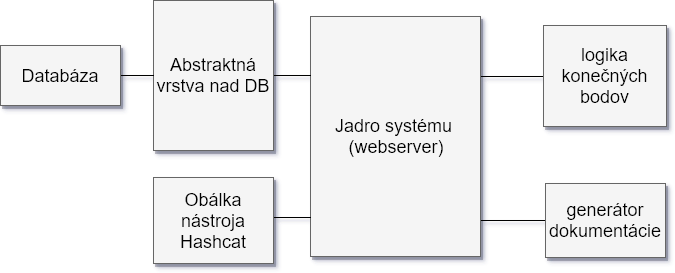
\includegraphics[scale=0.6]{obrazky/moduly.png}
    \caption{Rozdelenie systému do modulov}
    \label{fig:moduly}
\end{figure}

\subsubsection{Jadro systému}
Najhlavnejším modulom v~systéme je jeho jadro, ktoré spĺňa úlohu webového servera a sú v~ňom uložené nastavenia celého systému (prístupové údaje do databázy, zložka pre nahrávanie súborov, cesta k~nástroju Hashcat atď.). Pri zlyhaní jadra webový server odpovedá HTTP správy s~kódom začínajúcim číslom 5 (viď \ref{5XX}).


\subsubsection{Logika konečných bodov}
Jedná sa o~modul, v~ktorom sú obslúžené dotazy na konkrétne URI (viď. \ref{URI}). Zoznam dostupných URI je uvedený v~tabuľke (viď. \ref{zoznamURItable}). Väčšina konečných bodov podporuje viac typov HTTP metód (viď. \ref{httpMetody}). Podľa výberu metódy sa vykoná operácia so zdrojom. Niektoré konečné body podporujú takzvané query parametre za url adresou. Pri chybe v~tomto module, webový server odpovedá HTTP správami, ktoré začínajú číslom 4 (viď \ref{4XX}). Ak užívateľ žiada o~neplatnú kombináciu URI adresy a HTTP metódy, je mu vrátená HTTP správa s~kódom 404. V~prípade že je užívateľ neprihlásený a žiada o~zdroj, ktorý vyžaduje autentifikáciu, v~odpovedi dostane HTTP správu s~kódom 401. Pokiaľ je užívateľ prihlásený, ale na zdroj o~ktorý žiada nemá dostačujúce oprávnenia, tento modul vracia HTTP správu s~kódom 403. V~inakšom prípade je dotaz týmto modulom spracovaný. Ak nedôjde k~chybe počas spracovávania dotazu, modul vygeneruje odpoveď vo formáte JSON, ktorú pridá do tela HTTP odpovede s~kódom 200 (viď \ref{2XX}).


\begin{table}[h]
  \begin{center}
        \begin{tabular}{ |p{8cm}|p{7.4cm}|  }
         \hline
         Popis& URI\\
         \hline
          Operácie s kolekciou znakových sád & /charset/ \\
          Operácie s konkrétnou znakovou sadou & /charset/<id> \\
          Stiahnutie znakovej sady & /charset/<id>/download \\
          Operácie s kolekciou slovníkov & /dictionary/ \\
          Operácie s konskrétnym slovníkom & /dictionary/<id> \\
          Dáta na vykreslenie grafu podielu práce hostov & /graph/hostPercentage/<job\_id> \\
          Dáta na vykreslenie grafu vyťaženosti hostov & /graph/hostsComputing \\
          Dáta na vykreslenie grafu vyťaženosti hosta & /graph/hostsComputing/<id> \\
          Dáta na vykreslenie grafu progresu úloh & /graph/packagesProgress \\
          Dáta na vykreslenie grafu progresu úlohy & /graph/packagesProgress/<id> \\
          Útoky podporované nástrojom hashcat\ref{hashcat} & /hashcat/attackModes \\
          Typy hashov podporované nástrojom hashcat\ref{hashcat} & /hashcat/hashTypes \\
          Operácie s kolekciou hosťov & /hosts/ \\
           & /hosts/<id> \\
           & /hosts/info \\
           & /job/ \\
           & /job/<id> \\
           & /job/<id>/action \\
           & /job/<id>/host \\
           & /job/<id>/job \\
           & /job/crackingTime \\
           & /job/info \\
           & /job/verifyHash \\
           & /markovChains/ \\
           & /markovChains/<id> \\
           & /markovChains/makeFromDictionary \\
           & /masks/ \\
           & /masks/<id> \\
           & /masks/<id>/download \\
           & /masks/<id>/update \\
           & /notifications/ \\
           & /notifications/count \\
           & /protectedFiles/ \\
           & /protectedFiles/<id> \\
           & /rule/ \\
           & /rule/<id> \\
           & /rule/<id>/download \\
           & /serverInfo/control \\
           & /serverInfo/info \\
           & /user/ \\
           & /user/<id> \\
           & /user/isLoggedIn \\
           & /user/login \\
           & /user/logout \\
           & /user/role \\
           & /user/role/<id> \\
         \hline
        \end{tabular}
      \caption{Zoznam dostupných URI.}
      \label{zoznamURItable}
  \end{center}
\end{table}

\subsubsection{Obálka nástroja Hashcat}
Aj keď serverová časť systému Fitcrack nepoužíva priamo nástroj Hashcat na generovanie hešov kryptografických funkcií, používa ho na rôzne vedľajšie účely, ako napríklad získavanie podporovaných typov útokov a kryptografických hešov, alebo výpočet veľkosti množiny hesiel pre útok. Z~tohto dôvodu je potrebné implementovať obálku na tento nástroj vo forme objektu (triedy) s~požadovanými funkciami. To nám uľahčí prístup k~nástroju Hashcat a taktiež bezpečnejšie narábanie s~ním.

\subsubsection{Abstraktná vrstva nad databázou}
Jedná sa o~modul, ktorý uľahčuje prístup k~databáze. Zároveň výrazne neovplyvňuje výkon a flexibilitu systému. Vďaka tomu, že systém s~databázou nekomunikuje priamo, ale využíva abstraktnú vrstvu, je databáza lepšie chránená (ochrana pred útokmi typu SQL injection).


\subsubsection{Databáza}\label{navrhDB}
Vzhľadom nato, že systém Fitcrack využíva databázový server MySQL, rozhodol som sa napojiť na túto databázu. Aby bolo možné implementovať všetky rozšírenia systému, bude potrebné modifikovať štruktúru databázy. Na obrázku \ref{fig:ER} je možné vidieť entitno relačný diagram upravenej databázy. Zelenou farbou sú na ňom označené tabuľky, ktoré bude nutné do systému zaviesť. 

\begin{figure}[H]
    \centering
    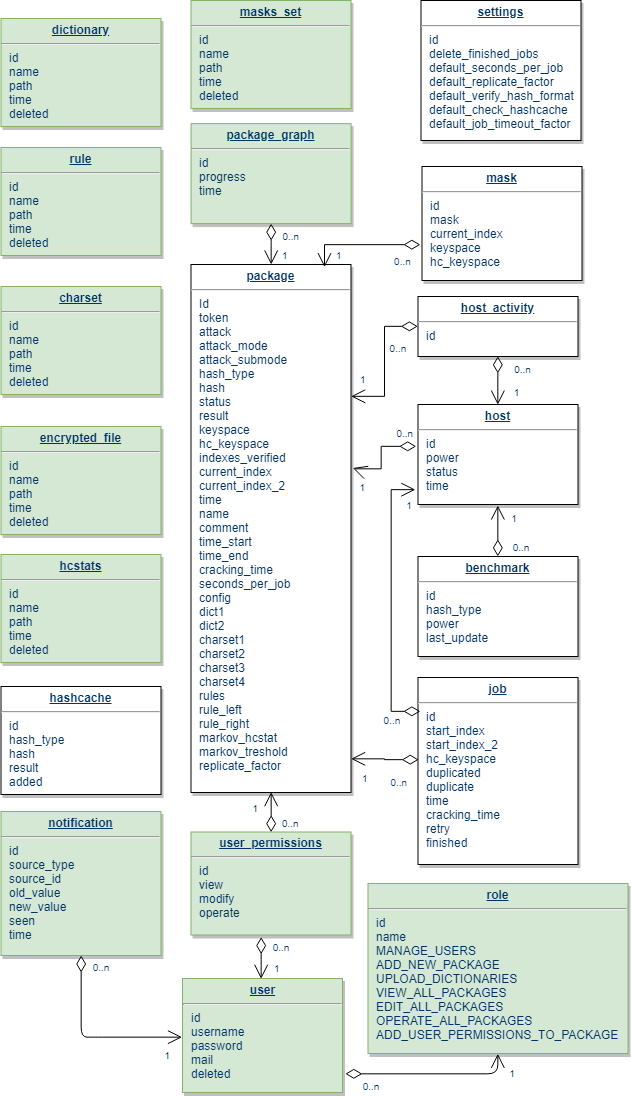
\includegraphics[scale=0.58]{obrazky/ER.PNG}
    \caption{Entitno-relačný diagram databázy. Zelenou farbou sú vyznačené nové tabuľky.}
    \label{fig:ER}
\end{figure}


\subsubsection{Generátor dokumentácie}
Generátor dokumentácie po spustení webového servera spracuje zdrojové kódy aj s~komentárami a vytvorí pomocou nich interaktívnu dokumentáciu (viď obr. \ref{fig:doc}). Z~nej je potom možné zistiť všetky dostupné koncové body spolu s~príkladmi odpovede. Generovanie dokumentácie automaticky nastáva aj pri zmene zdrojových súborov.

\begin{figure}[H]
    \centering
    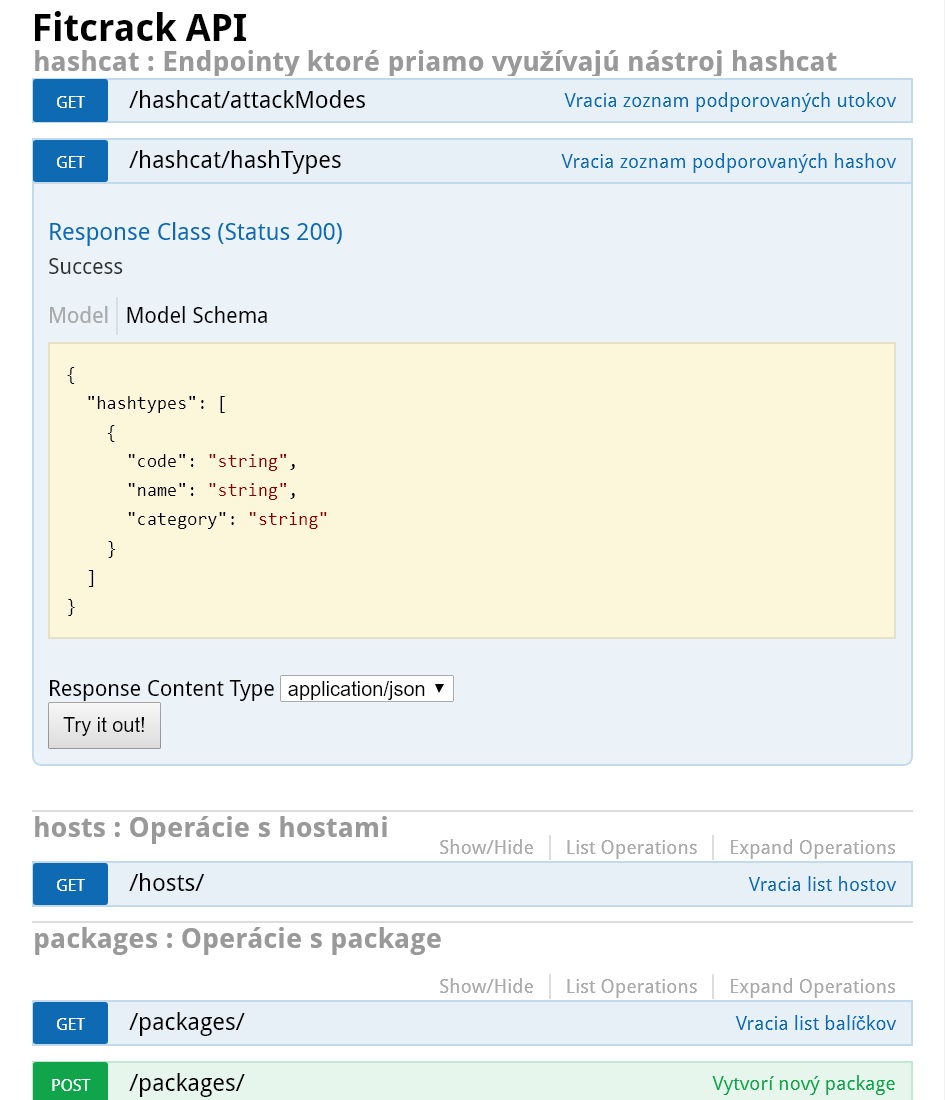
\includegraphics[scale=0.45]{obrazky/doc.PNG}
    \caption{Ukážka vygenerovanej dokumentácie}
    \label{fig:doc}
\end{figure}

\subsection{Autentifikácia a oprávnenia užívateľov}
Súčasná verzia systému Fitcrack nepodporuje viacerých užívateľov. Aby bolo možné do systému pridať užívateľov, je nutné rozšíriť databázu (viď. \ref{navrhDB}). Ako spôsob riešenia právomocí užívateľom som vybral systém oprávnení na základe rolí. Každý užívateľ bude mať uvedenú roľu, ktorá mu udeľuje právomoci na určité akcie. Jedná sa o jednoduchý systém, plne postačujúci pre menší počet užívateľov. Jednotlivé právomoci sú nasledujúce.


\begin{itemize}
    \item \textbf{Spravovanie užívateľov} - S takýmto oprávnením môže užívateľ vytvárať, mazať a modifikovať iných užívateľov.
    \item \textbf{Pridávanie novej úlohy} - Užívateľ môže pridať do systému novú úlohu
    \item \textbf{Nahrávanie súborov} - Užívateľ má oprávnenie do systému nahrať slovník, cudzojazyčné znakové sady, súbory s pravidlami, masky a súbory s markovými reťazcami. @TODO: Na všetko sa odkazovať do teórie
    \item \textbf{Zobrazenie všetkých úloh} - Užívateľ vidí v systéme všetky vytvorené úlohy.
    \item \textbf{Editovanie úloh} - Užívateľ môže všetky úlohy modifikovať.
    \item \textbf{Operácie s úlohami} - Užívateľ môže vykonávať s úlohami operácie štart, stop a reštart.
\end{itemize}





\section{Návrh klientskej časti}\label{navrhKlient}
Klientskú časť tvorí moderná webová aplikácia, ktorá pomocou HTTP žiadostí komunikuje so serverom (viď \ref{http}). Analýzou požiadavkov som zistil, že aplikácia by mala byť čo najlepšie ovládateľná a prehľadná pre užívateľa. Taktiež je veľmi dôležité, aby bol vzhľad stránky dobre štrukturovaný a pútavý. Aplikácia musí byť dostupná aj pre užívateľov s menším rozlíšením displeja ako klasický počítačový monitor. Z tohto dôvodu sa bude aplikácia prispôsobovať užívateľskému rozlíšeniu (responzívnosť).

Keďže je systém uzavretý a vyžaduje prihlasovanie, je vhodné, aby úvodná stránka aplikácie obsahovala prihlasovací formulár (viď obrázok \ref{fig:loginScreen}). Systém bude distribuovaný s jedným užívateľom v databáze, ktorý bude slúžiť na prvotné prihlásenie. Po prihlásení prostredníctvom tohoto užívateľa je možné vytvárať nových užívateľov vo vnútri aplikácie.




\begin{figure}[h]
\centering
\begin{minipage}{.5\textwidth}
    \centering
    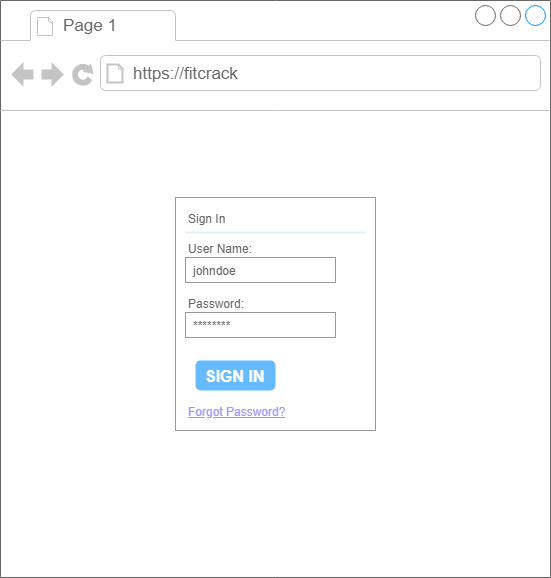
\includegraphics[width=0.95\linewidth]{obrazky/loginscreen.png}
    \caption{Návrh úvodnej stránky aplikácie.}
    \label{fig:loginScreen}
\end{minipage}%
\begin{minipage}{.5\textwidth}
    \centering
    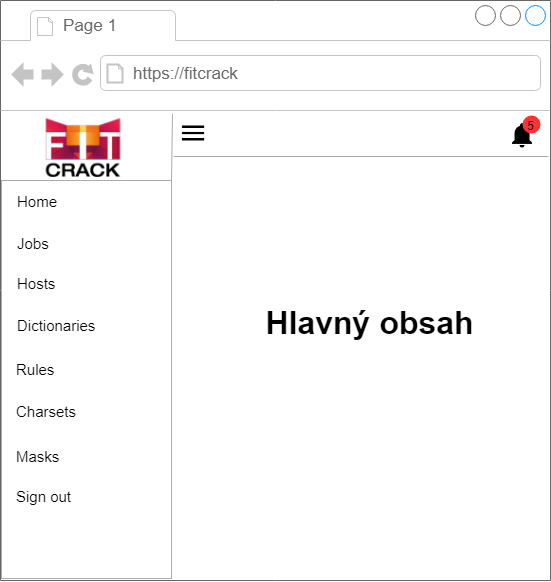
\includegraphics[width=0.95\linewidth]{obrazky/mainPage.png}
    \caption{Návrh úvodnej stránky aplikácie.}
    \label{fig:mainPage}\label{fig:mainPage}
\end{minipage}
\end{figure}

Všetky ostatné stránky tvorí jednotné rozhranie, ktoré sa skladá z postranného bočného panelu, hornej lišty a hlavného obsahu, ktorý je generický pre každú stránku. Tento bočný panel obsahuje logo Fitcracku, a navigáciu. Pre zachovanie responzívnosti celej aplikácie sa tento panel pri zariadeniach  s menším rozlíšením skryje, a zobrazí až po stlačení tlačítka Menu. Horná lišta obsahuje vľavo tlačítko Menu a napravo tlačítko Upozornenia, ktoré indikuje počet nových upozornení. Po stlačení tlačítka Upozornenia sa z pravej strany obrazovky vysunie panel s upozorneniami. Vďaka jednotnému rozmiestneniu navigačných prvkov pre všetky stránky, má užívateľ vždy prístup k všetkým rubrikám. Návrh štruktúry rozloženia stránky je možné vidieť na obrázku \ref{fig:mainPage}.


\section{Typy útokov v systéme Fitcrack}
V systéme Fitcrack je možné vytvárať päť druhov útokov. Pôvodný systém Fitcrack podporoval len dva základné. Každý útok je jedinečný a vhodný na iné situácie.


\subsection{Útok s maskami}
Jedná sa o útok hrubou silou. Užívateľ  vo webovej aplikácií zadá jednotlivé masky. Maska je textový reťazec pozostávajúci z pevne daných znakov a zástupných symbolov. Zástupné symboly sa označujú znakom ''\texttt{?}'' a symbolom znakovej sady. Napríklad mask \texttt{password?d} bude generovať heslá \texttt{password0 - password9}. Zabudované znakové sady v systéme sú nasledovné.
\begin{itemize}
    \item \textbf{?l} - znaková sada obsahuje malé písmená anglickej abecedy (abcdefghijklmnopqrstuvwxyz).
    \item \textbf{?u} - táto znaková sada obsahuje veľké písmená anglickej abecedy (ABCDEFGHIJKLMNOPQRSTUVWXYZ).
    \item \textbf{?d} - znaková sada obsahujúca arabské číslice (0123456789).
    \item \textbf{?h} - hexadecimálna znaková sada s malými písmenami (0123456789abcdef).
    \item \textbf{?H} - hexadecimálna znaková sada s veľkými písmenami (0123456789ABCDEF)
    \item \textbf{?s} - špeciálne znaky ako napríklad medzera !"\#\$\%\&
    '()*+,-./:;<=>?@
    \item \textbf{?a} - jedná sa o zjednotenie znakových sád ?l?u?d?s
    \item \textbf{?b} - v tejto znakovej sade sa nachádzajú všetky ASCII znaky (0x00 - 0xff).
\end{itemize}
V systéme je možné vybrať si až 4 ďalšie ľubovolné znakové sady k jednej úlohe. Tieto znakové sady sa potom zadávajú zástupnými symbolmi \texttt{?1 - ?4}.

Okrem znakových sád je možné pri útoku s maskami vybrať súbor s Markovými reťazcami. Tento súbor má zvyčajne príponu \texttt{.hcstat}, a je ho možné do systému nahrať, alebo vytvoriť analýzou slovníka s heslami priamo z prostredia webovej aplikácie. Jedná sa o súbor, v ktorom je uložená matica. Prvý stĺpec tejto matice obsahuje všetky znaky, z ktorých sa budú generovať heslá. Riadky matice sú usporiadané podľa pravdepodobnosti výskytu jednotlivých znakov. Príklad takejto matice je možné vidieť na obrázku \ref{fig:hcstatExample}. V prvom riadku matice sú znaky, ktorými najčastejšie začínajú heslá. Pri použití Markovho modelu sa negenerujú heslá postupne (napríklad pri použití masky \texttt{?l?l?l?l} sa negenerujú heslá v poradí \texttt{aaaa-zzzz}), ale práve podľa Markového modelu. Využitie tohto modelu pri generovaní hesiel je založené na pozorovaní, že ľudia pri tvorení hesiel používajú skrytý Markovský model. Pri vytváraní úlohy je možné taktiež určiť Markov prah, čo je kladné celé číslo, ktoré označuje do ktorého stĺpca v Markovom modely sa majú heslá generovať.

Tento útok už bol v systéme implementovaný. K útoku som pridal možnosť zadať znakové sady, Markovský model a možnosť načítať masky so súboru.


\begin{figure}[H]
  \centering
  \[
  \kbordermatrix{
      \\ 
      \varepsilon & n & p & s & u  & \dots  \\
      a & m & u & v & k & \dots \\
      b & i & y & e & u & \dots \\
      c & o & e & b & f & \dots \\
      \vdots & \vdots & \vdots & \vdots & \vdots & \vdots \\
      z & a & e & o & m  & \dots
  }
  \]
    \caption{Príklad Markovho modelu}
    \label{fig:hcstatExample}
\end{figure}

\subsection{Slovníkový útok}
Jeden z najzákladnejších útokov je útok pomocou slovníku, ktorý obsahuje veľký počet hesiel. Na každom riadku slovníka sa nachádza jedno heslo. Okrem slovníku je možné zvoliť aj súbor s pravidlami. Každé pravidlo sa aplikuje na každé heslo so slovníka. Pravidlá sú reťazce znakov. Majú pomerne jednoduchú syntax a umožňujú modifikovať heslo rôznymi spôsobmi \footnote{\url{https://hashcat.net/wiki/doku.php?id=rule_based_attack}}. Medzi základné pravidlá patria následovné znaky.
\begin{itemize}
    \item \textbf{l} - všetky písmená v hesle prevedie na malé písmená.
    \item \textbf{u} - prevedie prímená v hesle na veľké písmená.
    \item \textbf{t} - malé písmená prevedie na veľké a veľké na malé.
    \item \textbf{r} - otočí poradie písmen v hesle.
    \item \textbf{\$X} - na koniec hesla vloží znak X.
    \item \textbf{\^{}X} - na začiatok hesla vloží znak X. 
    \item \textbf{[} - zmaže prvý znak hesla.
    \item \textbf{]} - zmaže posledný znak hesla.
\end{itemize}
Pravidlá je možné medzi sebou aj kombinovať. Ak za každé heslo chceme pridať reťazec \texttt{123} a zároveň chceme každé heslo previesť na malé písmená, použijem pravidlo \texttt{l\$1\$2\$3}. V súbore s pravidlami sa môžu vyskytovať komentáre, ktoré začínajú znakom \texttt{\#}, a prázdne riadky.

Zjednodušená verzia tohto útoku, bez možnosti aplikovať pravidlá, bola v systéme už implementovaná.

\subsection{Kombinačný útok}
Pri kombinačnom útoku je nutné vybrať dva slovníky (ľavý a pravý). Každé heslo z ľavého slovníka sa skonkatenuje s každým heslom z pravého slovníka. Takto vznikajú nové heslá. Z každého hesla v ľavom slovníku vznikne toľko nových hesiel, koľko je hesiel v pravom slovníku. Ku každému slovníku je možné uviesť jedno pravidlo, ktoré upraví heslá v celom slovníku. Tento útok pôvodná webová aplikácia nepodporovala.

\subsection{Hybridné útoky}
Posledné typy útokov, ktoré moje riešenie podporuje sú hybridné útoky. Jedná sa o spojenie slovníkového útoku s útokom s použitím masky. Užívateľ si v systéme vyberie slovník a zadá masku. Potom sa maska so slovníkom skombinuje a vytvorí sa tak kombinačný útok. Napríklad, keď užívateľ zadá masku \texttt{?d} a vyberie slovník ktorý obsahuje heslá \texttt{aaa, bbb, ccc}, výsledná množina hesiel je 
\texttt{aaa0, aaa1, aaa2, aaa3, aaa4, aaa5, aaa6, aaa7, aaa8, aaa9, bbb0, ..., ccc9}. K maske aj slovníku je možné zadať jedno pravidlo. Hybridné útoky sú dva. Pri prvom je maska naľavo a slovník napravo, a pri druhom je slovník naľavo a maska napravo. Tento útok je nový v systéme Fitcrack.


\section{Grafy}
Keďže má byť nová aplikácia vizuálne prívetivá pre užívateľa, jej dôležitou súčasťou sú grafy. Navrhol som tri typy grafov.
\begin{itemize}
    \item \textbf{Graf progresu úlohy} \label{progressGraph} - tento graf je spojnicový a bude vykresľovať percentuálny pokrok jednej alebo viacerých úloh. Y-ová osa bude v percentách v rozmedzí 0 až 100. Na X-ovej osy bude čas. Tento graf zobrazuje koľko percent hesiel z celkovej množiny hesiel úlohy sa už skontrolovalo. Nezobrazuje progres hľadania hesla, keďže heslo môže byť nájdené hneď na začiatku množiny hesiel, alebo sa heslo nemusí nachádzať vôbec v množine hesiel danej úlohy.
    \item \textbf{Graf aktivity hosťov} - jedná sa taktiež o spojnicový graf, na ktorom je možné sledovať aktivitu jednotlivých hosťov. Na Y-ovej ose je možné vidieť počet kryptografických hešov, ktoré hosť počítal. Na X-ovej ose sa nachádza čas. Z tohto grafu by mala byť zrejmá aktivita Asimilátora (viď \ref{asimilator}), ktorý prispôsobuje počet hesiel v jednej pracovnej úlohe pre hosťa. Tento graf je možné zobraziť v rámci jednej úlohy, alebo v rámci systému.
    \item \textbf{Graf práce hosťov} - ide o koláčový graf, ktorý je možné zobraziť pre konkrétnu úlohu. Je z neho možné vyčítať množstvo práce jednotlivých hosťov v rámci úlohy.
\end{itemize}

\section{Notifikácie}
Ďalšou novinkou v systéme je systém notifikácií. Tieto notifikácie slúžia na upozornenie užívateľov pri zmene stavu úlohy. Sú rozdelené do niekoľkých kategórií - informačné, varovné, chybové a notifikácie úspechu. Vďaka tomu je možné notifikácie od seba aj vizuálne (farebne) odlíšiť. Medzi informačné notifikácie patria upozornenia o vytvorení úlohy, o spustení úlohy a o dokončovaní úlohy. Medzi notifikácie úspechu patrí upozornenia o nájdení hesla. Varovná notifikácie sa odošle v prípade že sa úloha zastavila z dôvodu nastavenia konca doby výpočtu pri vytváraní alebo editovaní úlohy, ale heslo sa ešte nenašlo. Chybová notifikácie nastáva po vyčerpaní celej množiny hesiel danej úlohy a nenájdení hesla.

Notifikácie obsahujú príznak videnia daným užívateľom. Tak tiež sa notifikácie o úlohách odosielajú len užívateľom, ktorí majú k danej úlohe oprávnenia.





\chapter{Implementácia}\label{implementacia}
Architektúru systému tvoria tri vrstvy - prezentačná, aplikačná a dátová (alebo databázová). Vrstvy medzi sebou spolupracujú a každá vrstva môže bežať na rôznej výpočetnej infraštruktúre. Architektúru systému je možné vidieť na obrázku \ref{fig:architektura}.
Prezentačná vrstva má za hlavnú úlohu komunikovať s aplikačnou vrstvou a vizualizovať dáta užívateľovi. Zobrazenie vo webovej prezentácii je implementované pomocou SPA (Single Page Application). Hlavnou úlohou SPA je synchronizácia stavu objektov medzi dátovou a prezentačnou vrstvou. 

Cieľom aplikačnej vrstvy aplikácie je spracovanie požiadavkov od prezentačnej vrstvy a komunikácia s databázovou vrstvou. Komunikácia s prezentačnou vrstvou prebieha vo formáte JSON.

Databázová vrstva tvorí MySQL databáza, ktorá je vytvorená podľa ER diagramu z obrázka \ref{fig:ER}. Databázová vrstva spracováva požiadavky aplikačnej vrstvy a vykonáva operácie ako ukladanie dát, zobrazovanie dát, vyhľadávanie a mazanie dát.

\begin{figure}[H]
    \centering
    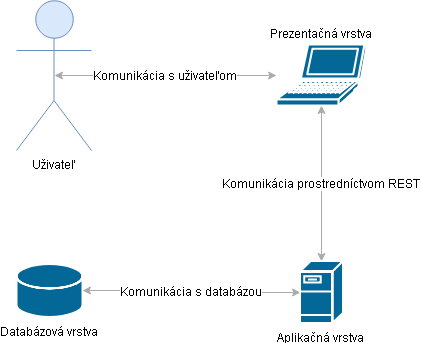
\includegraphics[scale=0.65]{obrazky/architektura.png}
    \caption{Architektúra aplikácie}
    \label{fig:architektura}
\end{figure}

\section{Implementácia databázovej vrstvy}
Databázová vrstva je implementovaná pomocou databázového systému MySQL. Je vytvorená podľa entitno relačného diagramu, ktorý je možné vidieť na obrázku \ref{fig:ER}. Tvoria ju pôvodné tabuľky systému Fitcrack a nové tabuľky, ktoré umožňujú implementáciu rozšírení systému. Tabuľky \texttt{dictionary}, \texttt{rule}, \texttt{masks\_set}, \texttt{hcstats} a \texttt{charset} slúžia na ukladanie informácii o súboroch nahratých do systému. Majú jednotnú štruktúru. Tvorí ju jednoznačný identifikátor záznamu v rámci tabuľky, názov súboru, cesta k súboru, čas pridania do databázy a príznak zmazania, ktorý slúži na signalizáciu aplikačnej vrstve, aby už súbor označený ako zmazaný, neposielala ďalej prezentačnej vrstve. Súbory označené ako zmazané ostávajú v systéme naďalej uložené kvôli predchádzaniu chýb v prípade že úloha, ktorá súbor využíva stále beží. Ďalšie nové tabuľky sú \texttt{user} a \texttt{role}, ktoré slúžia umožňujú autentifikáciu užívateľov a správu oprávnení. Pri užívateľoch sa ukladá ich prihlasovacie meno, heslo v zahešovanej podobe s pridanou soľou, email a odkaz do tabuľky \texttt{role}, ktorá obsahuje jednotlivé užívateľov oprávnenia v rámci systému. Oprávnenia k jednotlivým úloham môžu byť pridané prostredníctvom tabuľky \texttt{user\_permissions}. Tabuľka \texttt{notification} slúži na uchovávanie upozornení pre užívateľov. Údaje o progrese úloh sa uchovávajú v tabuľke \texttt{package\_graph}. Z týchto údajov je následne možné na prezentačnej vrstve vytvoriť graf progresu (viď \ref{progressGraph}). V databáze sa tiež nachádza triger, ktorý sa vykoná vždy po upravení úlohy. Tento triger je možné rozdeliť na dve časti. Prvá časť je možné vidieť na výpise \ref{progressTriger} a slúži na počítanie progresu úlohy a pridávanie záznamov do tabuľky \texttt{package\_graph}.
\begin{algorithm}
  \caption{Telo trigeru, ktorý pridáva záznamy do tabuľky \texttt{package\_graph}.}
  \label{progressTriger}
  \begin{lstlisting}[
             language=SQL,
             showspaces=false,
             basicstyle=\ttfamily,
             numbers=left,{}
          ]
-- verified passwords changed
IF NEW.indexes_verified <> OLD.indexes_verified THEN
  INSERT INTO package_graph (progress, package_id) VALUES (
    -- if job finished or exhausted set progress to 100. 
    -- Else calculate progress.
    IF(NEW.hc_keyspace = 0 OR NEW.status = 1 OR NEW.status = 2,
      100,
      ROUND((NEW.indexes_verified / NEW.hc_keyspace) * 100, 2)
    ),
    NEW.id  
  );
END IF;
  \end{lstlisting}
\end{algorithm}
 Druhá časť trigeru je vyobrazená na výpise \ref{notificationTrigger}. Slúži na rozosielanie notifikácií užívateľom. Je dôležité aby triger vybral len tých užívateľov, ktorí majú k úlohe prístup (užívatelia s roľou, ktorá má oprávnenie na zobrazenie všetkých úloh, alebo užívatelia s oprávnením k úlohe v tabuľke \texttt{user\_permissions}).
\begin{algorithm}[H]
  \caption{Trigger, ktorý má na starosti rozposielanie notifikácií užívateľom.}
  \label{notificationTrigger}
  \begin{lstlisting}[
             language=SQL,
             showspaces=false,
             basicstyle=\ttfamily,
             numbers=left,{}
          ]
IF NEW.status <> OLD.status THEN 
  OPEN userWithPermissionCursor; 
    user_loop: LOOP
      FETCH userWithPermissionCursor INTO user_idCursor;
        IF done THEN LEAVE user_loop; END IF;
      INSERT INTO fc_notification 
        VALUES user_id, source_id, old_value, new_value
        (user_idCursor, NEW.id, OLD.status, NEW.status);
    END LOOP;
  CLOSE userWithPermissionCursor;
END IF;
  \end{lstlisting}
\end{algorithm}

\section{Implementácia aplikačnej vrstvy}
Aplikačná vrstva je implementovaná v prostredí Python3. Tvorí ju sada balíkov, ktoré plnia rozličné úlohy. Adresárovú štruktúru je možné vidieť na obrázku \ref{fig:serverStructure}.
\begin{figure}[H]
\begin{center}
\begin{varwidth}{\linewidth}
\begin{verbatim}
\---src
    +---api
    |   \---fitcrack
    |       +---attacks
    |       \---endpoints
    |           +---charset
    |           +---dictionary
    |           +---graph
    |           +---hashcat
    |           +---host
    |           +---markov
    |           +---masks
    |           +---notifications
    |           +---package
    |           +---protectedFile
    |           +---rule
    |           +---serverInfo
    |           \---user
    \---database
\end{verbatim}
\end{varwidth}
\end{center}
\caption{Hierarchia balíčkov aplikačnej vrstvy.}
\label{fig:serverStructure}
\end{figure}
V koreňovom adresári sa nachádza súbor \texttt{app.py}, ktorý obsahuje funkciu \texttt{main()}. Táto funkcie najprv prevedie inicializáciu systému, systém nakonfiguruje a načíta všetky koncové body aplikačného rozhrania, a následne spustí webový server. O chod webevého servera sa stará framework Flask. Ďalší dôležitý súbor v koreňovom adresári je \texttt{settings.py}, ktorý slúži na nastavenie servera. Je v ňom možné nakonfigurovať cestu k databázovému systému, debugovací režim, adresu a číslo portu servera. Tiež obsahuje cesty k zložkám na ukladanie slovníkov, Markovských modelov, cudzojazyčných znakových sád, súborov s pravidlami a zašifrovaných súborov. Ďalej sa v tomto súbore nachádzajú cesty k rôznym pomocným programom, ktoré systém využíva. Jedná sa o program Hashcat (viď \ref{hashcat}), MaskProcessor\footnote{\url{https://hashcat.net/wiki/doku.php?id=maskprocessor}}, XtoHashcat\footnote{\url{https://fitcrack.fit.vutbr.cz/?i=download}} a HashValidator\footnote{\url{https://github.com/Zippersk/hashValidator}}. Koreňový adresár obsahuje jediný balík s názvom \texttt{src}, v ktorom sú ďalšie balíky \texttt{database} a \texttt{api}. Balík \texttt{database} obsahuje modul s názvom \texttt{models.py}, ktorý má na starosti mapovanie databázy na abstraktný databázový model. Tento súbor obsahuje triedy, ktoré predstavujú jednotlivé tabuľky z databázy. Príklad takejto triedy je možné vidieť na výpise \ref{abstractDBClass}. 
\begin{algorithm}
  \caption{Trieda, ktorá predstavuje mapovanie na databázovú tabuľku.}
  \label{abstractDBClass}
  \begin{lstlisting}[
             language=Python,
             showspaces=false,
             basicstyle=\ttfamily,
             numbers=left,{}
          ]
class FcPackageGraph(Base):
    __tablename__ = 'fc_package_graph'

    id = Column(BigInteger, primary_key=True)
    progress = Column(Numeric(5, 2), nullable=False)
    package_id = Column(ForeignKey('fc_package.id'), nullable=False, index=True)
    time = Column(DateTime, server_default=text("CURRENT_TIMESTAMP"))

    package = relationship('FcPackage')

    def as_graph(self):
        return {
            'time': str(getattr(self, 'time')),
            getattr(self.package, 'id'): round(getattr(self, 'progress'))
        }
  \end{lstlisting}
\end{algorithm}
Tieto triedy boli vytvorené prostredníctvom programu sqlacodegen\footnote{\url{https://pypi.org/project/sqlacodegen/1.1.0/}}. Abstraktná vrstva nad databázou výrazne uľahčuje manipuláciu s databázovými objektami. K triedam je možné doimplementovať hybridné vlastnosti, ktoré bývajú zvyčajne vyjadrené na základe stĺpcov odpovedajúcej tabuľky. Napríklad, keďže je nájdené heslo pri úlohe uložené v stĺpci \texttt{result} vo formáte Base64\footnote{\url{https://sk.wikipedia.org/wiki/Base64}}, je možné vytvoriť hybridnú vlastnosť triedy, ktorá automaticky po načítaní dát z databázy dekóduje heslo uložené vo formáte Base64 a priradí ho do hybridnej vlastnosti. Abstraktná vrstva databázy je implementovaná prostredníctvom frameworku SQLalchemy.

\subsection{Implementácia jednotlivých zdrojov}


\subsection{Spracovanie útokov}
Spracovanie jednotlivých útokov prebieha v balíčku \texttt{attacks}

\chapter{Záver}\label{zaver}
V~tejto práci sa mi podarilo navrhnúť implementáciu serverovej časti systému Fitcrack s~automaticky generovanou dokumentáciou. Zameral som sa na vylepšenia súčasnej verzie webového prostredia Fitcracku a navrhol som rozšírenia, ku príkladu systém viacerých užívateľov, ktoré spríjemnia užívateľom používanie. Taktiež som odstránil nedokonalosti súčasného riešenia, ako napríklad dostupnosť len z~webovej platformy. Systém, implementovaný podľa môjho návrhu bude dostupný zo všetkých platforiem, ktoré sú schopné sieťovej komunikácie. Súčasne sa zníži záťaž na server, pretože bude prerozdelená medzi klienta a server. Vďaka implementácie pomocou modulov bude celý systém ľahko rozšíriteľný. Návrh opísaný v~tejto práci tiež ošetruje niekoľko bezpečnostných dier súčasnej implementácie. Návrh spĺňa všetky zásady architektúry REST (viď \ref{zasadyREST}), a taktiež je vhodný na testovacie účely systému.

Keďže som v~rámci tejto práce zhromaždil potrebné znalosti, v~nasledujúcom semestri budem pracovať na implementácií navrhnutého systému. Tiež sa budem venovať testovaniu spoľahlivosti a experimentom. Systém podrobím výkonnostným testom a výsledky porovnám so súčasným riešením. 
Mojou snahou je vytvoriť aplikačné rozhranie na vzdialené ovládanie systému Fitcrack takým spôsobom, aby implementácia klientskej časti užívateľského rozhrania bola jednoduchá a vyžadovala čo najmenej informácií o~štruktúre serverovej časti. 






  % Pouzita literatura / Bibliography
  % ----------------------------------------------
\ifslovak
  \makeatletter
  \def\@openbib@code{\addcontentsline{toc}{chapter}{Literatúra}}
  \makeatother
  \bibliographystyle{bib-styles/czechiso}
\else
  \ifczech
    \makeatletter
    \def\@openbib@code{\addcontentsline{toc}{chapter}{Literatura}}
    \makeatother
    \bibliographystyle{bib-styles/czechiso}
  \else 
    \makeatletter
    \def\@openbib@code{\addcontentsline{toc}{chapter}{Bibliography}}
    \makeatother
    \bibliographystyle{bib-styles/englishiso}
  %  \bibliographystyle{alpha}
  \fi
\fi
  \begin{flushleft}
  \bibliography{projekt-20-literatura-bibliography}
  \end{flushleft}

  % vynechani stranky v oboustrannem rezimu
  % Skip the page in the two-sided mode
  \iftwoside
    \cleardoublepage
  \fi

  % Prilohy / Appendices
  % ---------------------------------------------
  \appendix
\ifczech
  \renewcommand{\appendixpagename}{Přílohy}
  \renewcommand{\appendixtocname}{Přílohy}
  \renewcommand{\appendixname}{Příloha}
\fi
\ifslovak
  \renewcommand{\appendixpagename}{Prílohy}
  \renewcommand{\appendixtocname}{Prílohy}
  \renewcommand{\appendixname}{Príloha}
\fi
%  \appendixpage

% vynechani stranky v oboustrannem rezimu
% Skip the page in the two-sided mode
%\iftwoside
%  \cleardoublepage
%\fi
  
\ifslovak
%  \section*{Zoznam príloh}
%  \addcontentsline{toc}{section}{Zoznam príloh}
\else
  \ifczech
%    \section*{Seznam příloh}
%    \addcontentsline{toc}{section}{Seznam příloh}
  \else
%    \section*{List of Appendices}
%    \addcontentsline{toc}{section}{List of Appendices}
  \fi
\fi
  \startcontents[chapters]
  \setlength{\parskip}{0pt}
  % seznam příloh / list of appendices
  % \printcontents[chapters]{l}{0}{\setcounter{tocdepth}{2}}
  
  \ifODSAZ
    \setlength{\parskip}{0.5\bigskipamount}
  \else
    \setlength{\parskip}{0pt}
  \fi
  
  % vynechani stranky v oboustrannem rezimu
  \iftwoside
    \cleardoublepage
  \fi
  
  % Přílohy / Appendices
  %% Tento soubor nahraďte vlastním souborem s přílohami (nadpisy níže jsou pouze pro příklad)
% This file should be replaced with your file with an appendices (headings below are examples only)

% Umístění obsahu paměťového média do příloh je vhodné konzultovat s vedoucím
% Placing of table of contents of the memory media here should be consulted with a supervisor
%\chapter{Obsah přiloženého paměťového média}

%\chapter{Manuál}

%\chapter{Konfigurační soubor} % Configuration file

%\chapter{RelaxNG Schéma konfiguračního souboru} % Scheme of RelaxNG configuration file

%\chapter{Plakát} % poster

\chapter{Jak pracovat s touto šablonou}
\label{jak}

V této kapitole je uveden popis jednotlivých částí šablony, po kterém následuje stručný návod, jak s touto šablonou pracovat. 

Jedná se o přechodnou verzi šablony. Nová verze bude zveřejněna do~konce roku 2017 a~bude navíc obsahovat nové pokyny ke správnému využití šablony, závazné pokyny k~vypracování bakalářských a diplomových prací (rekapitulace pokynů, které jsou dostupné na~webu) a nezávazná doporučení od vybraných vedoucích, která již teď najdete na~webu (viz odkazy v souboru s literaturou). Jediné soubory, které se v nové verzi změní, budou \texttt{projekt-01-kapitoly-chapters.tex} a \texttt{projekt-30-prilohy-appendices.tex}, jejichž obsah každý student vymaže a nahradí vlastním. Šablonu lze tedy bez problémů využít i~v~současné verzi.

\section*{Popis částí šablony}

Po rozbalení šablony naleznete následující soubory a adresáře:
\begin{DESCRIPTION}
  \item [bib-styles] Styly literatury (viz níže). 
  \item [obrazky-figures] Adresář pro Vaše obrázky. Nyní obsahuje placeholder.pdf (tzv. TODO obrázek, který lze použít jako pomůcku při tvorbě technické zprávy), který se s prací neodevzdává. Název adresáře je vhodné zkrátit, aby byl jen ve zvoleném jazyce.
  \item [template-fig] Obrázky šablony (znak VUT).
  \item [fitthesis.cls] Šablona (definice vzhledu).
  \item [Makefile] Makefile pro překlad, počítání normostran, sbalení apod. (viz níže).
  \item [projekt-01-kapitoly-chapters.tex] Soubor pro Váš text (obsah nahraďte).
  \item [projekt-20-literatura-bibliography.bib] Seznam literatury (viz níže).
  \item [projekt-30-prilohy-appendices.tex] Soubor pro přílohy (obsah nahraďte).
  \item [projekt.tex] Hlavní soubor práce -- definice formálních částí.
\end{DESCRIPTION}

Výchozí styl literatury (czechiso) je od Ing. Martínka, přičemž anglická verze (englishiso) je jeho překladem s drobnými modifikacemi. Oproti normě jsou v něm určité odlišnosti, ale na FIT je dlouhodobě akceptován. Alternativně můžete využít styl od Ing. Radima Loskota nebo od Ing. Radka Pyšného\footnote{BP Ing. Radka Pyšného \url{http://www.fit.vutbr.cz/study/DP/BP.php?id=7848}}. Alternativní styly obsahují určitá vylepšení, ale zatím nebyly řádně otestovány větším množstvím uživatelů. Lze je považovat za beta verze pro zájemce, kteří svoji práci chtějí mít dokonalou do detailů a neváhají si nastudovat detaily správného formátování citací, aby si mohli ověřit, že je vysázený výsledek v pořádku.

Makefile kromě překladu do PDF nabízí i další funkce:
\begin{itemize}
  \item přejmenování souborů (viz níže),
  \item počítání normostran,
  \item spuštění vlny pro doplnění nezlomitelných mezer,
  \item sbalení výsledku pro odeslání vedoucímu ke kontrole (zkontrolujte, zda sbalí všechny Vámi přidané soubory, a případně doplňte).
\end{itemize}

Nezapomeňte, že vlna neřeší všechny nezlomitelné mezery. Vždy je třeba manuální kontrola, zda na konci řádku nezůstalo něco nevhodného -- viz Internetová jazyková příručka\footnote{Internetová jazyková příručka \url{http://prirucka.ujc.cas.cz/?id=880}}.

\paragraph {Pozor na číslování stránek!} Pokud má obsah 2 strany a na 2. jsou jen \uv{Přílohy} a~\uv{Seznam příloh} (ale žádná příloha tam není), z nějakého důvodu se posune číslování stránek o 1 (obsah \uv{nesedí}). Stejný efekt má, když je na 2. či 3. stránce obsahu jen \uv{Literatura} a~je možné, že tohoto problému lze dosáhnout i jinak. Řešení je několik (od~úpravy obsahu, přes nastavení počítadla až po sofistikovanější metody). \textbf{Před odevzdáním proto vždy překontrolujte číslování stran!}


\section*{Doporučený postup práce se šablonou}

\begin{enumerate}
  \item \textbf{Zkontrolujte, zda máte aktuální verzi šablony.} Máte-li šablonu z předchozího roku, na stránkách fakulty již může být novější verze šablony s~aktualizovanými informacemi, opravenými chybami apod.
  \item \textbf{Zvolte si jazyk}, ve kterém budete psát svoji technickou zprávu (česky, slovensky nebo anglicky) a svoji volbu konzultujte s vedoucím práce (nebyla-li dohodnuta předem). Pokud Vámi zvoleným jazykem technické zprávy není čeština, nastavte příslušný parametr šablony v souboru projekt.tex (např.: \verb|documentclass[english]{fitthesis}| a přeložte prohlášení a poděkování do~angličtiny či slovenštiny.
  \item \textbf{Přejmenujte soubory.} Po rozbalení je v šabloně soubor \texttt{projekt.tex}. Pokud jej přeložíte, vznikne PDF s technickou zprávou pojmenované \texttt{projekt.pdf}. Když vedoucímu více studentů pošle \texttt{projekt.pdf} ke kontrole, musí je pracně přejmenovávat. Proto je vždy vhodné tento soubor přejmenovat tak, aby obsahoval Váš login a (případně zkrácené) téma práce. Vyhněte se však použití mezer, diakritiky a speciálních znaků. Vhodný název může být např.: \uv{\texttt{xlogin00-Cisteni-a-extrakce-textu.tex}}. K přejmenování můžete využít i přiložený Makefile:
\begin{verbatim}
make rename NAME=xlogin00-Cisteni-a-extrakce-textu
\end{verbatim}
  \item Vyplňte požadované položky v souboru, který byl původně pojmenován \texttt{projekt.tex}, tedy typ, rok (odevzdání), název práce, svoje jméno, ústav (dle zadání), tituly a~jméno vedoucího, abstrakt, klíčová slova a další formální náležitosti.
  \item Nahraďte obsah souborů s kapitolami práce, literaturou a přílohami obsahem svojí technické zprávy. Jednotlivé přílohy či kapitoly práce může být výhodné uložit do~samostatných souborů -- rozhodnete-li se pro toto řešení, je doporučeno zachovat konvenci pro názvy souborů, přičemž za číslem bude následovat název kapitoly. 
  \item Nepotřebujete-li přílohy, zakomentujte příslušnou část v \texttt{projekt.tex} a příslušný soubor vyprázdněte či smažte. Nesnažte se prosím vymyslet nějakou neúčelnou přílohu jen proto, aby daný soubor bylo čím naplnit. Vhodnou přílohou může být obsah přiloženého paměťového média.
  \item Nascanované zadání uložte do souboru \texttt{zadani.pdf} a povolte jeho vložení do práce parametrem šablony v projekt.tex (\verb|documentclass[zadani]{fitthesis}|).
  \item Nechcete-li odkazy tisknout barevně (tedy červený obsah -- bez konzultace s vedoucím nedoporučuji), budete pro tisk vytvářet druhé PDF s tím, že nastavíte parametr šablony pro tisk: (\verb|documentclass[zadani,print]{fitthesis}|).  Barevné logo se nesmí tisknout černobíle!
  \item Vzor desek, do kterých bude práce vyvázána, si vygenerujte v informačním systému fakulty u zadání. Pro disertační práci lze zapnout parametrem v šabloně (více naleznete v souboru fitthesis.cls).
  \item Nezapomeňte, že zdrojové soubory i (obě verze) PDF musíte odevzdat na CD či jiném médiu přiloženém k technické zprávě.
\end{enumerate}

Obsah práce se generuje standardním příkazem \tt \textbackslash tableofcontents \rm (zahrnut v šabloně). Přílohy jsou v něm uvedeny úmyslně.

\subsection*{Pokyny pro oboustranný tisk}
\begin{itemize}
\item \textbf{Oboustranný tisk je doporučeno konzultovat s vedoucím práce.}
\item Je-li práce tištěna oboustranně a její tloušťka je menší než tloušťka desek, nevypadá to dobře.
\item Zapíná se parametrem šablony: \verb|\documentclass[twoside]{fitthesis}|
\item Po vytištění oboustranného listu zkontrolujte, zda je při prosvícení sazební obrazec na obou stranách na stejné pozici. Méně kvalitní tiskárny s duplexní jednotkou mají často posun o 1--3 mm. Toto může být u některých tiskáren řešitelné tak, že vytisknete nejprve liché stránky, pak je dáte do stejného zásobníku a vytisknete sudé.
\item Za titulním listem, obsahem, literaturou, úvodním listem příloh, seznamem příloh a případnými dalšími seznamy je třeba nechat volnou stránku, aby následující část začínala na liché stránce (\textbackslash cleardoublepage).
\item  Konečný výsledek je nutné pečlivě překontrolovat.
\end{itemize}

\subsection*{Styl odstavců}

Odstavce se zarovnávají do bloku a pro jejich formátování existuje více metod. U papírové literatury je častá metoda s~použitím odstavcové zarážky, kdy se u~jednotlivých odstavců textu odsazuje první řádek odstavce asi o~jeden až dva čtverčíky (vždy o~stejnou, předem zvolenou hodnotu), tedy přibližně o~dvě šířky velkého písmene M základního textu. Poslední řádek předchozího odstavce a~první řádek následujícího odstavce se v~takovém případě neoddělují svislou mezerou. Proklad mezi těmito řádky je stejný jako proklad mezi řádky uvnitř odstavce. \cite{fitWeb} Další metodou je odsazení odstavců, které je časté u elektronické sazby textů. První řádek odstavce se při této metodě neodsazuje a mezi odstavce se vkládá vertikální mezera o~velikosti 1/2 řádku. Obě metody lze v kvalifikační práci použít, nicméně často je vhodnější druhá z uvedených metod. Metody není vhodné kombinovat.

Jeden z výše uvedených způsobů je v šabloně nastaven jako výchozí, druhý můžete zvolit parametrem šablony \uv{\tt odsaz\rm }.

\subsection*{Užitečné nástroje}
\label{nastroje}

Následující seznam není výčtem všech využitelných nástrojů. Máte-li vyzkoušený osvědčený nástroj, neváhejte jej využít. Pokud však nevíte, který nástroj si zvolit, můžete zvážit některý z následujících:

\begin{description}
	\item[\href{http://miktex.org/download}{MikTeX}] \LaTeX{} pro Windows -- distribuce s jednoduchou instalací a vynikající automatizací stahování balíčků.
	\item[\href{http://texstudio.sourceforge.net/}{TeXstudio}] Přenositelné opensource GUI pro \LaTeX{}.  Ctrl+klik umožňuje přepínat mezi zdrojovým textem a PDF. Má integrovanou kontrolu pravopisu, zvýraznění syntaxe apod. Pro jeho využití je nejprve potřeba nainstalovat MikTeX.
	\item[\href{http://www.winedt.com/}{WinEdt}] Ve Windows je dobrá kombinace WinEdt + MiKTeX. WinEdt je GUI pro Windows, pro jehož využití je nejprve potřeba nainstalovat \href{http://miktex.org/download}{MikTeX} či \href{http://www.tug.org/texlive/}{TeX Live}. 
	\item[\href{http://kile.sourceforge.net/}{Kile}] Editor pro desktopové prostředí KDE (Linux). Umožňuje živé zobrazení náhledu. Pro jeho využití je potřeba mít nainstalovaný \href{http://www.tug.org/texlive/}{TeX Live} a Okular. 
	\item[\href{http://jabref.sourceforge.net/download.php}{JabRef}] Pěkný a jednoduchý program v Javě pro správu souborů s bibliografií (literaturou). Není potřeba se nic učit -- poskytuje jednoduché okno a formulář pro editaci položek.
	\item[\href{https://inkscape.org/en/download/}{InkScape}] Přenositelný opensource editor vektorové grafiky (SVG i PDF). Vynikající nástroj pro tvorbu obrázků do odborného textu. Jeho ovládnutí je obtížnější, ale výsledky stojí za to.
	\item[\href{https://git-scm.com/}{GIT}] Vynikající pro týmovou spolupráci na projektech, ale může výrazně pomoci i jednomu autorovi. Umožňuje jednoduché verzování, zálohování a přenášení mezi více počítači.
	\item[\href{http://www.overleaf.com/}{Overleaf}] Online nástroj pro \LaTeX{}. Přímo zobrazuje náhled a umožňuje jednoduchou spolupráci (vedoucí může průběžně sledovat psaní práce), vyhledávání ve zdrojovém textu kliknutím do PDF, kontrolu pravopisu apod. Zdarma jej však lze využít pouze s určitými omezeními (někomu stačí na disertaci, jiný na ně může narazit i při psaní bakalářské práce) a pro dlouhé texty je pomalejší.
\end{description}

Pozn.: Overleaf nepoužívá Makefile v šabloně -- aby překlad fungoval, je nutné kliknout pravým tlačítkem na \tt projekt.tex \rm a zvolit \uv{Set as Main File}.


\subsection*{Užitečné balíčky pro \LaTeX}

Studenti při sazbě textu často řeší stejné problémy. Některé z nich lze vyřešit následujícími balíčky pro \LaTeX:

\begin{itemize}
  \item \verb|amsmath| -- rozšířené možnosti sazby rovnic,
  \item \verb|float, afterpage, placeins| -- úprava umístění obrázků,
  \item \verb|fancyvrb, alltt| -- úpravy vlastností prostředí Verbatim, 
  \item \verb|makecell| -- rozšíření možností tabulek,
  \item \verb|pdflscape, rotating| -- natočení stránky o 90 stupňů (pro obrázek či tabulku),
  \item \verb|hyphenat| -- úpravy dělení slov,
  \item \verb|picture, epic, eepic| -- přímé kreslení obrázků.
\end{itemize}

Některé balíčky jsou využity přímo v šabloně (v dolní části souboru fitthesis.cls). Nahlédnutí do jejich dokumentace může být rovněž užitečné.

Sloupec tabulky zarovnaný vlevo s pevnou šířkou je v šabloně definovaný \uv{L} (používá se jako \uv{p}).


  
  % Kompilace po částech (viz výše, nutno odkomentovat)
  % Compilation piecewise (see above, it is necessary to uncomment it)
  %\subfile{projekt-30-prilohy-appendices}
  
\end{document}
